% generated by Plantuml 1.2024.2       
\definecolor{plantucolor0000}{RGB}{0,0,0}
\definecolor{plantucolor0001}{RGB}{241,241,241}
\definecolor{plantucolor0002}{RGB}{24,24,24}
\definecolor{plantucolor0003}{RGB}{235,147,127}
\definecolor{plantucolor0004}{RGB}{200,41,48}
\definecolor{plantucolor0005}{RGB}{132,190,132}
\definecolor{plantucolor0006}{RGB}{3,128,72}
\definecolor{plantucolor0007}{RGB}{180,167,229}
\definecolor{plantucolor0008}{RGB}{173,209,178}
\definecolor{plantucolor0009}{RGB}{242,77,92}
\scalebox{0.6}{
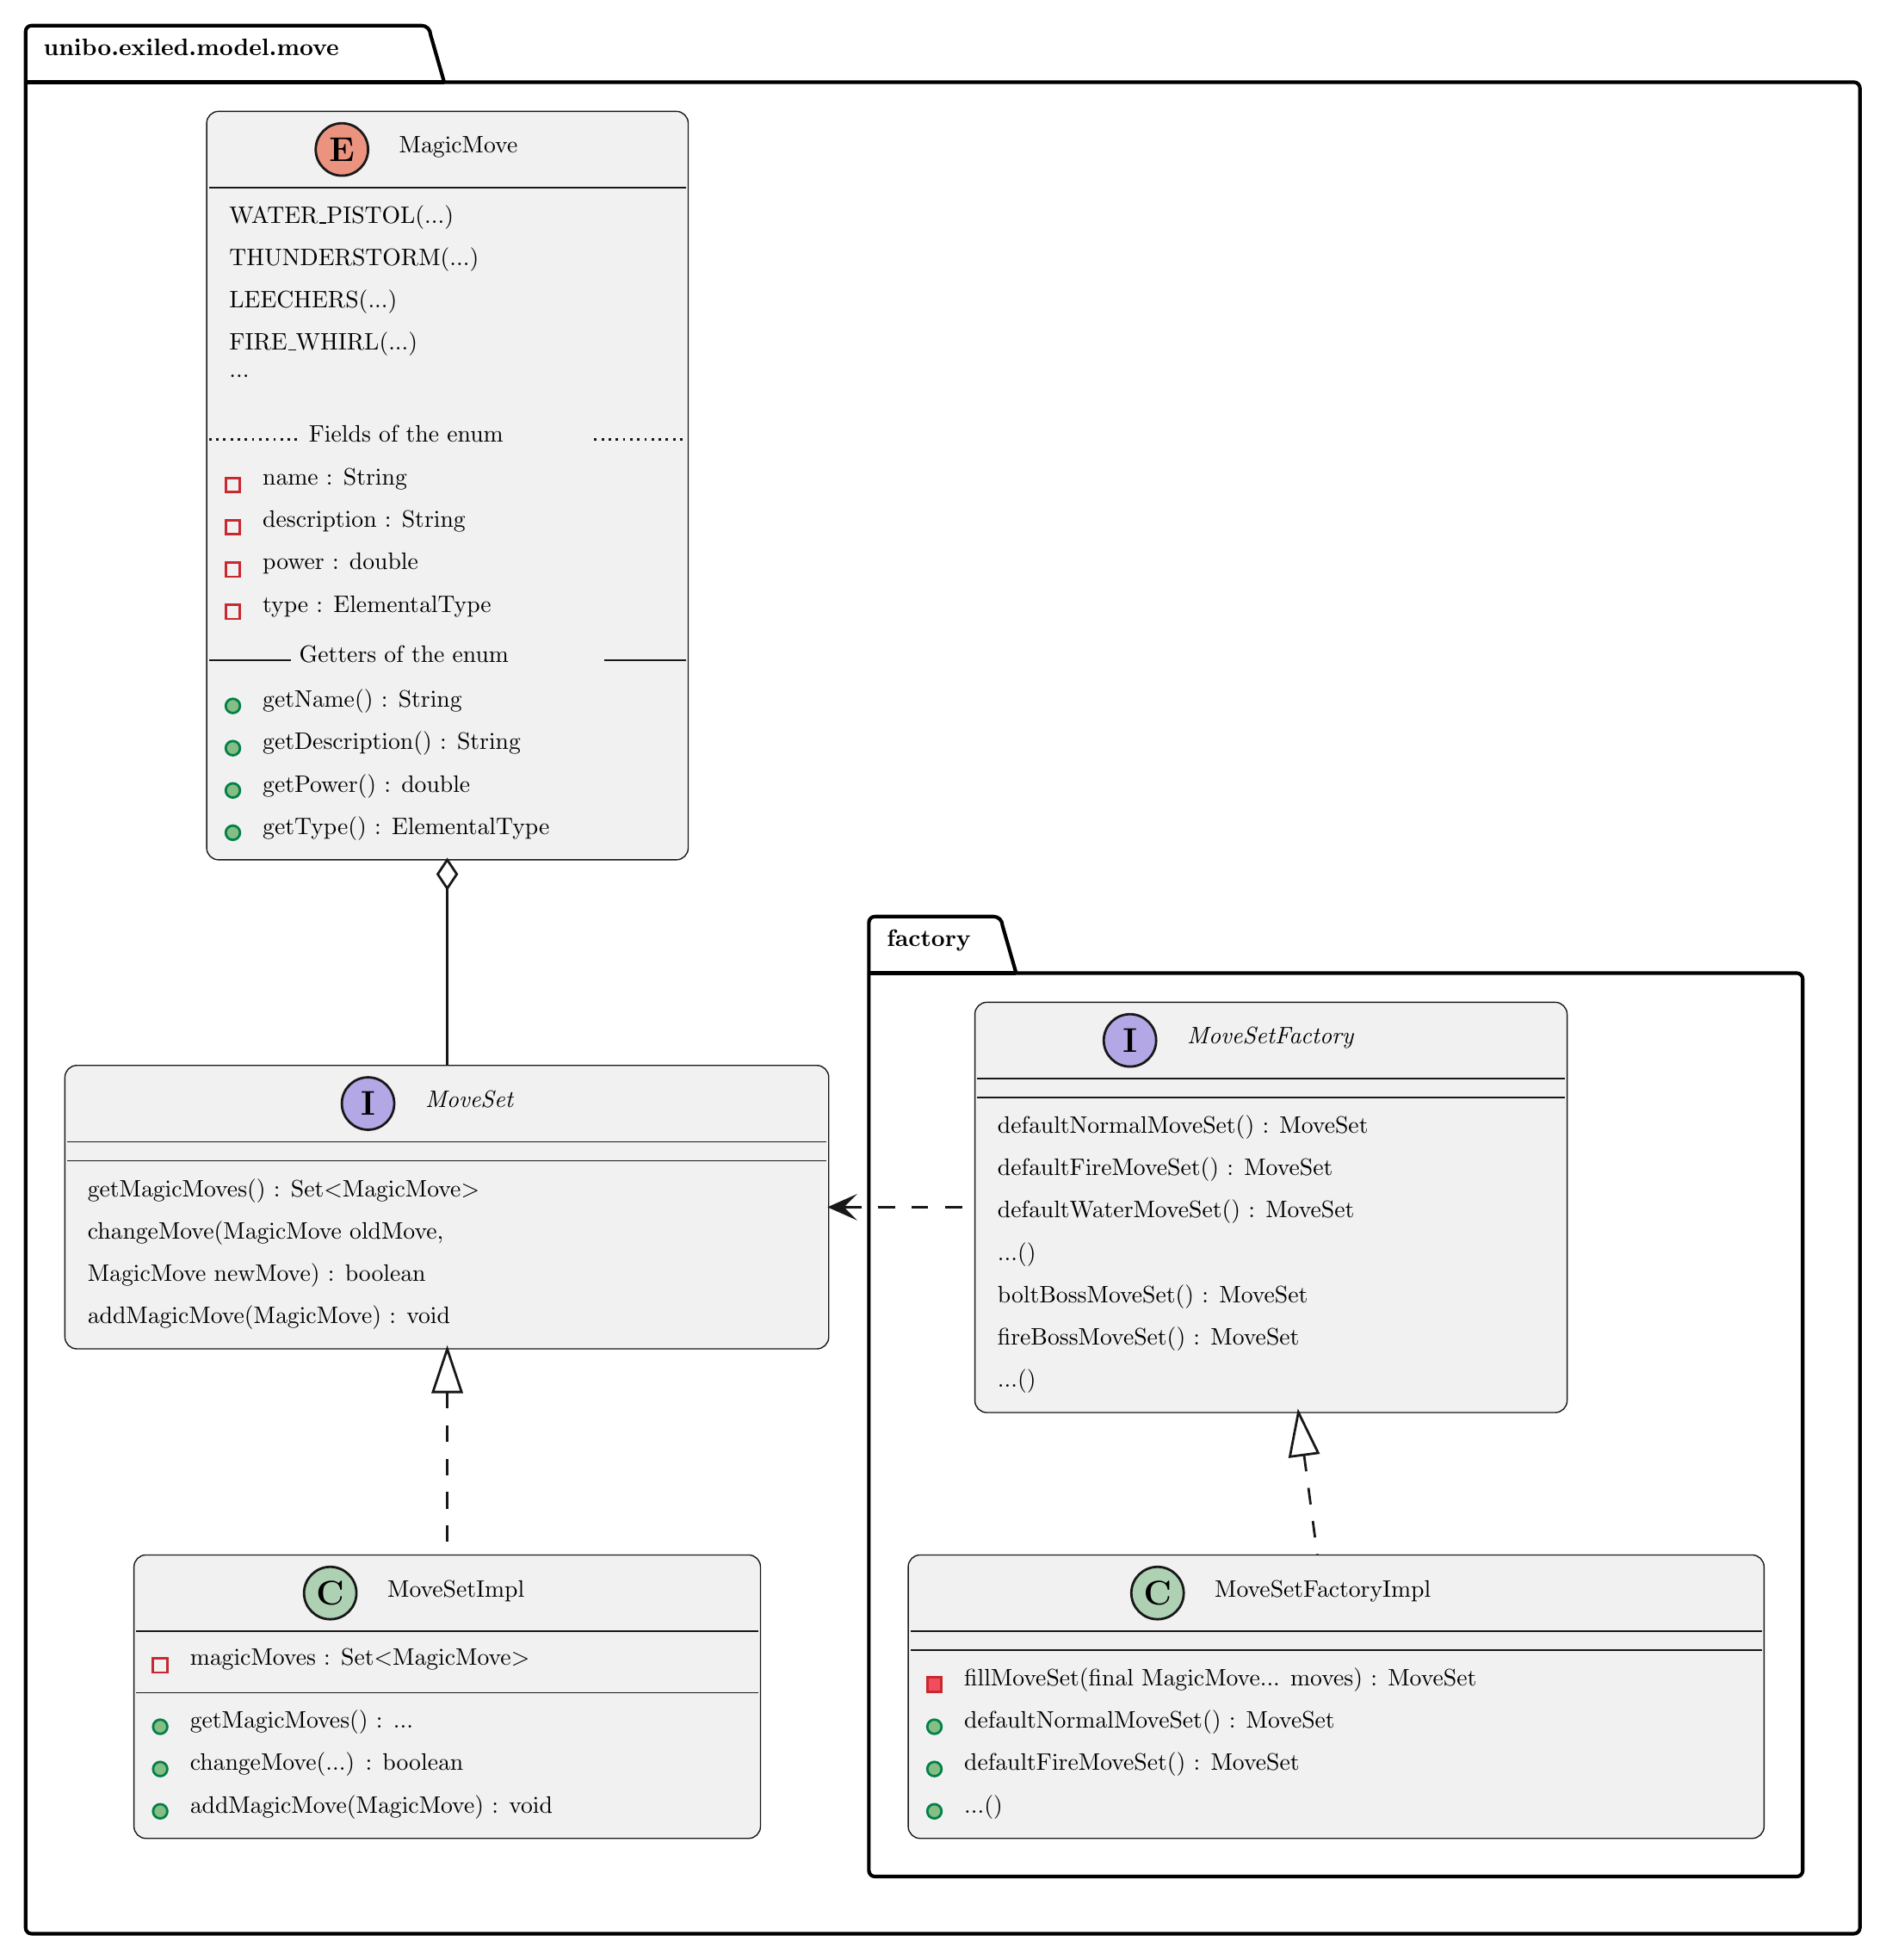
\begin{tikzpicture}[yscale=-1
,pstyle0/.style={color=black,line width=1.5pt}
,pstyle1/.style={color=plantucolor0002,fill=plantucolor0001,line width=0.5pt}
,pstyle3/.style={color=plantucolor0002,line width=0.5pt}
,pstyle4/.style={color=plantucolor0004,line width=1.0pt}
,pstyle5/.style={color=plantucolor0002,line width=1.0pt,dash pattern=on 1.0pt off 2.0pt}
,pstyle6/.style={color=plantucolor0006,fill=plantucolor0005,line width=1.0pt}
,pstyle7/.style={color=plantucolor0002,fill=plantucolor0007,line width=1.0pt}
,pstyle8/.style={color=plantucolor0002,fill=plantucolor0008,line width=1.0pt}
,pstyle10/.style={color=plantucolor0002,line width=1.0pt,dash pattern=on 7.0pt off 7.0pt}
,pstyle11/.style={color=plantucolor0002,line width=1.0pt}
]
\draw[pstyle0] (8.5pt,6pt) -- (172.2158pt,6pt) arc(270:360:3.75pt)  -- (181.7158pt,29.7461pt) -- (773.5pt,29.7461pt) arc(270:360:2.5pt)  -- (776pt,804.5pt) arc(0:90:2.5pt)  -- (8.5pt,807pt) arc(90:180:2.5pt)  -- (6pt,8.5pt) arc(180:270:2.5pt) ;
\draw[pstyle0] (6pt,29.7461pt) -- (181.7158pt,29.7461pt);
\node at (10pt,8pt)[below right,color=black]{\textbf{unibo.exiled.model.move}};
\draw[pstyle0] (362.5pt,380pt) -- (412.3093pt,380pt) arc(270:360:3.75pt)  -- (421.8093pt,403.7461pt) -- (749.5pt,403.7461pt) arc(270:360:2.5pt)  -- (752pt,780.5pt) arc(0:90:2.5pt)  -- (362.5pt,783pt) arc(90:180:2.5pt)  -- (360pt,382.5pt) arc(180:270:2.5pt) ;
\draw[pstyle0] (360pt,403.7461pt) -- (421.8093pt,403.7461pt);
\node at (364pt,382pt)[below right,color=black]{\textbf{factory}};
\draw[pstyle1] (82pt,47pt) arc (180:270:5pt) -- (87pt,42pt) -- (279.16pt,42pt) arc (270:360:5pt) -- (284.16pt,47pt) -- (284.16pt,351.1914pt) arc (0:90:5pt) -- (279.16pt,356.1914pt) -- (87pt,356.1914pt) arc (90:180:5pt) -- (82pt,351.1914pt) -- cycle;
\draw[color=plantucolor0002,fill=plantucolor0003,line width=1.0pt] (138.7793pt,58pt) ellipse (11pt and 11pt);
\node at (138.7793pt,58pt)[]{\textbf{\Large E}};
\node at (159.2793pt,49.127pt)[below right,color=black]{MagicMove};
\draw[pstyle3] (83pt,74pt) -- (283.16pt,74pt);
\node at (88pt,78pt)[below right,color=black]{WATER\_PISTOL(...)};
\node at (88pt,95.7461pt)[below right,color=black]{THUNDERSTORM(...)};
\node at (88pt,113.4922pt)[below right,color=black]{LEECHERS(...)};
\node at (88pt,131.2383pt)[below right,color=black]{FIRE\_WHIRL(...)};
\node at (88pt,148.9844pt)[below right,color=black]{...};
\draw[pstyle4] (90pt,195.8496pt) rectangle (96pt,201.8496pt);
\node at (102pt,188.4766pt)[below right,color=black]{name : String};
\draw[pstyle4] (90pt,213.5957pt) rectangle (96pt,219.5957pt);
\node at (102pt,206.2227pt)[below right,color=black]{description : String};
\draw[pstyle4] (90pt,231.3418pt) rectangle (96pt,237.3418pt);
\node at (102pt,223.9688pt)[below right,color=black]{power : double};
\draw[pstyle4] (90pt,249.0879pt) rectangle (96pt,255.0879pt);
\node at (102pt,241.7148pt)[below right,color=black]{type : ElementalType};
\draw[pstyle5] (83pt,179.6035pt) -- (121.4133pt,179.6035pt);
\node at (121.4133pt,170.2305pt)[below right,color=black]{Fields of the enum};
\draw[pstyle5] (244.7467pt,179.6035pt) -- (283.16pt,179.6035pt);
\draw[pstyle6] (93pt,291.5801pt) ellipse (3pt and 3pt);
\node at (102pt,281.207pt)[below right,color=black]{getName() : String};
\draw[pstyle6] (93pt,309.3262pt) ellipse (3pt and 3pt);
\node at (102pt,298.9531pt)[below right,color=black]{getDescription() : String};
\draw[pstyle6] (93pt,327.0723pt) ellipse (3pt and 3pt);
\node at (102pt,316.6992pt)[below right,color=black]{getPower() : double};
\draw[pstyle6] (93pt,344.8184pt) ellipse (3pt and 3pt);
\node at (102pt,334.4453pt)[below right,color=black]{getType() : ElementalType};
\draw[pstyle3] (83pt,272.334pt) -- (117.3508pt,272.334pt);
\node at (117.3508pt,262.9609pt)[below right,color=black]{Getters of the enum};
\draw[pstyle3] (248.8092pt,272.334pt) -- (283.16pt,272.334pt);
\draw[pstyle1] (22.5pt,447.5pt) arc (180:270:5pt) -- (27.5pt,442.5pt) -- (338.1519pt,442.5pt) arc (270:360:5pt) -- (343.1519pt,447.5pt) -- (343.1519pt,556.4844pt) arc (0:90:5pt) -- (338.1519pt,561.4844pt) -- (27.5pt,561.4844pt) arc (90:180:5pt) -- (22.5pt,556.4844pt) -- cycle;
\draw[pstyle7] (149.7474pt,458.5pt) ellipse (11pt and 11pt);
\node at (149.7474pt,458.5pt)[]{\textbf{\Large I}};
\node at (170.2474pt,449.627pt)[below right,color=black]{\textit{MoveSet}};
\draw[pstyle3] (23.5pt,474.5pt) -- (342.1519pt,474.5pt);
\draw[pstyle3] (23.5pt,482.5pt) -- (342.1519pt,482.5pt);
\node at (28.5pt,486.5pt)[below right,color=black]{getMagicMoves() : Set\textless MagicMove\textgreater };
\node at (28.5pt,504.2461pt)[below right,color=black]{changeMove(MagicMove oldMove,};
\node at (28.5pt,521.9922pt)[below right,color=black]{                     MagicMove newMove) : boolean};
\node at (28.5pt,539.7383pt)[below right,color=black]{addMagicMove(MagicMove) : void};
\draw[pstyle1] (51.5pt,653pt) arc (180:270:5pt) -- (56.5pt,648pt) -- (309.491pt,648pt) arc (270:360:5pt) -- (314.491pt,653pt) -- (314.491pt,761.9844pt) arc (0:90:5pt) -- (309.491pt,766.9844pt) -- (56.5pt,766.9844pt) arc (90:180:5pt) -- (51.5pt,761.9844pt) -- cycle;
\draw[pstyle8] (133.8823pt,664pt) ellipse (11pt and 11pt);
\node at (133.8823pt,664pt)[]{\textbf{\Large C}};
\node at (154.3823pt,655.127pt)[below right,color=black]{MoveSetImpl};
\draw[pstyle3] (52.5pt,680pt) -- (313.491pt,680pt);
\draw[pstyle4] (59.5pt,691.373pt) rectangle (65.5pt,697.373pt);
\node at (71.5pt,684pt)[below right,color=black]{magicMoves : Set\textless MagicMove\textgreater };
\draw[pstyle3] (52.5pt,705.7461pt) -- (313.491pt,705.7461pt);
\draw[pstyle6] (62.5pt,720.1191pt) ellipse (3pt and 3pt);
\node at (71.5pt,709.7461pt)[below right,color=black]{getMagicMoves() : ...};
\draw[pstyle6] (62.5pt,737.8652pt) ellipse (3pt and 3pt);
\node at (71.5pt,727.4922pt)[below right,color=black]{changeMove(...) : boolean};
\draw[pstyle6] (62.5pt,755.6113pt) ellipse (3pt and 3pt);
\node at (71.5pt,745.2383pt)[below right,color=black]{addMagicMove(MagicMove) : void};
\draw[pstyle1] (404.5pt,421pt) arc (180:270:5pt) -- (409.5pt,416pt) -- (648.103pt,416pt) arc (270:360:5pt) -- (653.103pt,421pt) -- (653.103pt,583.2227pt) arc (0:90:5pt) -- (648.103pt,588.2227pt) -- (409.5pt,588.2227pt) arc (90:180:5pt) -- (404.5pt,583.2227pt) -- cycle;
\draw[pstyle7] (469.5902pt,432pt) ellipse (11pt and 11pt);
\node at (469.5902pt,432pt)[]{\textbf{\Large I}};
\node at (490.0902pt,423.127pt)[below right,color=black]{\textit{MoveSetFactory}};
\draw[pstyle3] (405.5pt,448pt) -- (652.103pt,448pt);
\draw[pstyle3] (405.5pt,456pt) -- (652.103pt,456pt);
\node at (410.5pt,460pt)[below right,color=black]{defaultNormalMoveSet() : MoveSet};
\node at (410.5pt,477.7461pt)[below right,color=black]{defaultFireMoveSet() : MoveSet};
\node at (410.5pt,495.4922pt)[below right,color=black]{defaultWaterMoveSet() : MoveSet};
\node at (410.5pt,513.2383pt)[below right,color=black]{...()};
\node at (410.5pt,530.9844pt)[below right,color=black]{boltBossMoveSet() : MoveSet};
\node at (410.5pt,548.7305pt)[below right,color=black]{fireBossMoveSet() : MoveSet};
\node at (410.5pt,566.4766pt)[below right,color=black]{...()};
\draw[pstyle1] (376.5pt,653pt) arc (180:270:5pt) -- (381.5pt,648pt) -- (730.7678pt,648pt) arc (270:360:5pt) -- (735.7678pt,653pt) -- (735.7678pt,761.9844pt) arc (0:90:5pt) -- (730.7678pt,766.9844pt) -- (381.5pt,766.9844pt) arc (90:180:5pt) -- (376.5pt,761.9844pt) -- cycle;
\draw[pstyle8] (481.1673pt,664pt) ellipse (11pt and 11pt);
\node at (481.1673pt,664pt)[]{\textbf{\Large C}};
\node at (501.6673pt,655.127pt)[below right,color=black]{MoveSetFactoryImpl};
\draw[pstyle3] (377.5pt,680pt) -- (734.7678pt,680pt);
\draw[pstyle3] (377.5pt,688pt) -- (734.7678pt,688pt);
\draw[color=plantucolor0004,fill=plantucolor0009,line width=1.0pt] (384.5pt,699.373pt) rectangle (390.5pt,705.373pt);
\node at (396.5pt,692pt)[below right,color=black]{fillMoveSet(final MagicMove... moves) : MoveSet};
\draw[pstyle6] (387.5pt,720.1191pt) ellipse (3pt and 3pt);
\node at (396.5pt,709.7461pt)[below right,color=black]{defaultNormalMoveSet() : MoveSet};
\draw[pstyle6] (387.5pt,737.8652pt) ellipse (3pt and 3pt);
\node at (396.5pt,727.4922pt)[below right,color=black]{defaultFireMoveSet() : MoveSet};
\draw[pstyle6] (387.5pt,755.6113pt) ellipse (3pt and 3pt);
\node at (396.5pt,745.2383pt)[below right,color=black]{...()};
\draw[pstyle10] (183pt,579.59pt) ..controls (183pt,606.71pt) and (183pt,620.86pt) .. (183pt,647.97pt);
\draw[pstyle11] (183pt,561.59pt) -- (177pt,579.59pt) -- (189pt,579.59pt) -- (183pt,561.59pt) -- cycle;
\draw[pstyle10] (542.6631pt,605.9629pt) ..controls (545.3431pt,626.1129pt) and (545.76pt,629.32pt) .. (548.24pt,647.98pt);
\draw[pstyle11] (540.29pt,588.12pt) -- (536.7155pt,606.7539pt) -- (548.6108pt,605.1718pt) -- (540.29pt,588.12pt) -- cycle;
\draw[pstyle10] (349.84pt,502pt) ..controls (369.97pt,502pt) and (384.1pt,502pt) .. (404.23pt,502pt);
\draw[color=plantucolor0002,fill=plantucolor0002,line width=1.0pt] (343.84pt,502pt) -- (352.84pt,506pt) -- (348.84pt,502pt) -- (352.84pt,498pt) -- (343.84pt,502pt) -- cycle;
\draw[pstyle11] (183pt,368.23pt) ..controls (183pt,399.01pt) and (183pt,417.46pt) .. (183pt,442.44pt);
\draw[pstyle11] (183pt,356.23pt) -- (179pt,362.23pt) -- (183pt,368.23pt) -- (187pt,362.23pt) -- (183pt,356.23pt) -- cycle;
\end{tikzpicture}
}
